\documentclass{article}

\usepackage{xeCJK, indentfirst, geometry}
\usepackage{hyperref}
\usepackage{booktabs}

\geometry{a4paper}

%\setCJKmainfont{微软雅黑}

\title{Project Report of RISCV-CPU}
\author{Yi Gu}

\begin{document}
    \maketitle

    \section{Summary}

        This project is a RISC-V CPU with five-stage pipeline, implemented in Verilog HDL.

        The CPU can be simulated by Icarus Verilog or Xilinx xsim, and can be implemented on Basys3 FPGA, using Xilinx vivado.

        The repository of this project may be found at: \url{https://github.com/wu-qing-157/RISCV-CPU}.

    \section{Design}

        \subsection{Project Overview}

            This project has a standard $5$-stage pipeline with some additional features, and the overview structure is shown in the below figure:

            \begin{center}
                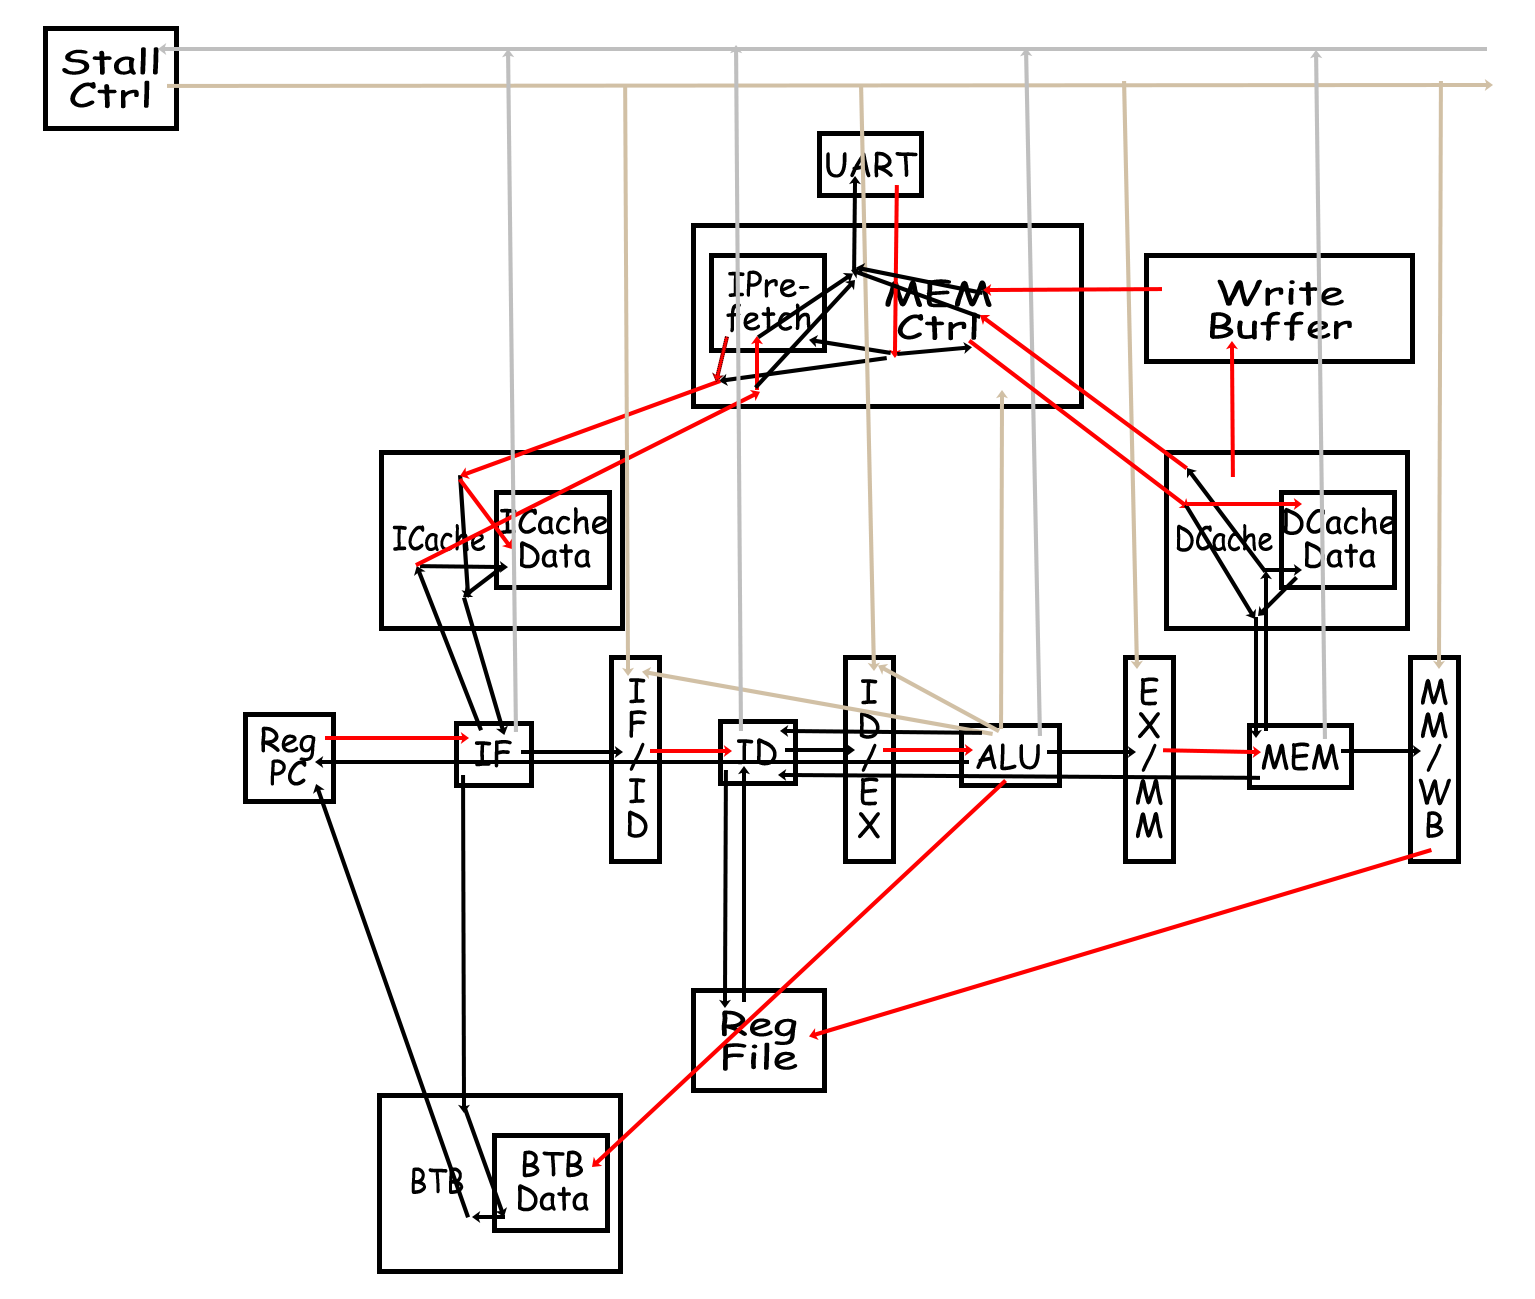
\includegraphics[scale=0.7]{Overview.png}
            \end{center}

            Note: Red lines represent data flow controlled by clock.
            Lines with light color represent control flow.

        \subsection{Features}
            
            Main features implemented in this project are listed as below, with some of them described in later part of this section.

            \begin{table}[h]
            \centering
            \begin{tabular}{l l}
                \toprule
                Feature & Description\\
                \midrule
                ISA & RV32I subset of RISC-V\\
                Pipelining & Standard 5 stages\\
                Data Forwarding & Complete forwarding paths\\
                Cache & Direct mapping Instruction Cache \& Direct mapping Data Cache\\
                Write Buffer & $1$-block $4$-byte Write Buffer\\
                Branch Prediction & $2$-bit Branch Target Buffer\\
                IF Prefetch & Prefetch during spare time of memory port\\
                \bottomrule
            \end{tabular}
            \end{table}

            Details of some features are listed below:

            \begin{description}
                \item[Instruction Cache]
                    A direct mapping I-Cache with size of $256 \times 4~\mathrm{bytes}$ is implemented.
                    If cache hits, the data will be returned in the same cycle,
                    while, otherwise, fetching of the instruction will be started from the next cycle.
                    The slow behavior of cache-hit check and memory port is to blame for the additional cycle.
                    The latency caused by the additional cycle is eliminated with \textit{IF Prefetch} described below.
                \item[Data Cache]
                    A direct mapping D-Cache with size of $128 \times 4~\mathrm{bytes}$ is implemented.
                    The write policy is a mixture of write back and write through,
                    and in detail, $4$-byte store insructions use write back and other store instructions use write through.
                    It is so arranged because of the large proportion of $4$-byte store instructions,
                    and the $4$-byte block size due to limitation of units on FPGA.
                    Similar as I-Cache, cache-hit data is returned in the same cycle, while cache-misses take an addtional cycle.
                \item[Write Buffer]
                    A naive single-block $4$-byte write buffer is added for D-Cache.
                    Data in write buffer will be flushed when memory port is not busy.
                \item[IF Prefetch]
                    After an instruction is fetched, the next instruction will be pre-fetched.
                    The prioity of the pre-fetching is lower than load needed by D-Cache, but higher than write buffer.
                    Note that in this implementation, I-Cache-miss and D-Cache-miss takes $3$ unused cycles,
                    the pre-fetching will also take advantage of these $3$ cycles, with exception described in next section.
                    Note that \textit{IF Prefetch} will be interrupted by wrong branch predition (prefetching is meaningless),
                    or branches predicted taken (cache-hit rate of the target instruction is very high).
            \end{description}

        \subsection{Performance}
            
            The implemented CPU can be run on FPGA with a frequency of $230~\mathrm{MHz}$.

            It can pass all tests on FPGA listed in the project repository.
            Note that it has some problems during simulation due to some issues in the given \textit{hci.v}.

            Some detailed performance quota are tested based on testcases in the project repository.

    \clearpage

            \begin{table}[h]
            \centering
            \begin{tabular}{l c c c c}
                \toprule
                Testname & Instructions & Cycles & CPI & FPGA Time (sec)\\
                \midrule
                bulgarian & $872042$ & $955046$ & $1.095$ & - \\
                pi & - & - & - & $0.469$ \\
                magic & $661360$ & $723539$ & $1.094$ & $0.031$ \\
                queens & $521577$ & $585617$ & $1.123$ & $0.563$ \\
                love & - & - & - & $183.3$\\
                \bottomrule
            \end{tabular}
            \end{table}

    \section{Thinkings}

        \begin{description}
            \item[Issues in given files]
                In the given files, there does exist lots of issues disturbing my finishing this project.
                When testing with simulation, some bytes written to IO port will be displayed twice or even four times.
                In order to check who is to blame, I need to check the huge wave grapth.
                Reading from IO port will cause last reading from memory port invalid,
                and the reading address one cycle after reading from IO port must have $1$ on its $17$-th bit
                to keep the IO reading valid.
                These two issues disturb me a lot when debugging my project on FPGA.
                I think as a course project, the above $3$ issues are supposed not happen,
                and we students should at least be informed.
                However, the assignment repository and TAs give me a bad feel.
                Addtionally, due to the issues mentioned above,
                the \textit{IF Prefetch} will be interrupted by a IO reading, and will be restarted after next IF reading.
            \item[The motivation for \textit{IF Prefetch} and \textit{Write Buffer}]
                The memory port on FPGA is completely different from RAM in modern computer,
                where the motivation for \textit{IF Prefetch} and \textit{Write Buffer} comes from.
                \textit{Write Buffer} dalays unimportant write behavior to gaps between reading,
                and \textit{IF Prefetch} makes full use of the actually unused cycles.
                Based on simulation tests, it's better to grant \textit{IF Prefetch} a higher priority than \textit{Write Buffer}.
            \item[The block size of Cache]
                Due to the limitation of units on FPGA, the way of memory access,
                and the proportion of $4$-byte load instructions, as well as the difficulties in implementation,
                $4$-byte block size is chosen for both I-Cache and D-Cache.
            \item[Mapping method of Cache and BTB]
                The performance on FPGA is not so good for me to choose
                fully-associated or set-associated. Actually, even implemented as direct mapping,
                I-Cache-hit and D-Cache-hit are the bottleneck of the performance.
            \item[Total size of Cache and BTB]
                Currently I have $256$ blocks for I-Cache, $128$ blocks for D-Cache,
                and $32$ blocks for BTB.
                As tested, the CPI performance can only increase by less than $0.5\%$ if I double any of it,
                so these $3$ figures are chosen.
%            \item[Annoying grading standard]
%                Also it seems inappropriate to include this part in a project report,
%                I still want to make complaints about the quite annoying grading standard.
%                The grading standard of this course project is neither given in time nor being paricular.
%                The standard was specified near the deadline, not granting us sufficient time to achieve some grades.
%                It was also vague on point assignments, which may cause dispute on final grading.
%                Besides that, TAs informed us of the bonus of presentation just during the week filled with final exams.
%                At least, it was too late. The presentation should not be assigned on last week, especially a busy week.
%                Also, the bonus of presentation is itself improper.
%                From my point of view, it should be either nonexistent or required to everyone, but may not be treated as a bonus.
        \end{description}

    \section{Acknowledgement}

        Special thanks would go to Yuan Yao and Zonghan Yang who discuss with me some features implemented in this project,
        and Haichen Dong who informed me of the issues in given files.
        Also, I would like to express my gratitude to TAs
        for providing codes for memory and IO ports (although with some issued).
        I also referenced the book \textit{自己动手写 CPU} and Zhou Fan's project at the very beginning of my own project.

    \section*{Reference}

        \begin{itemize}
            \item 雷思磊. \textit{自己动手写CPU}, 电子工业出版社, 2014
            \item Zhou Fan. RISC-V-CPU. \url{https://github.com/Evensgn/RISC-V-CPU}
        \end{itemize}
\end{document}
